\chapter{The preprocessing of social media data}
\label{chap:mining}
 
The mainstream adoption of the Internet has changed the landscape of
information diffusion. Nowadays, we can use a lot of resources existing
on the internet such as the news broadcasting from the news media
websites (e.g. CNN, NY Times) to the personal blog and the
rumor/information spreading from the SNS (e.g. Facebook,
Twitter). Almost all the data we collected from the news media
websites or SNS are in text format. To describe the information
diffusion, there are three basic things we need know: the diffusing
information, the directed link to describe who infect whom, the time
when the diffusion happened. Thus, when analyzing the information
diffusion, the first step for us is to extract the topological
structure, which expresses the relationship among the entities
(i.e. the research objects, such as the person and the blog), and the
useful attributes.  For the information diffusion, the attributes that
we are interested in are usually the topics of the diffused
information, the timestamp at which one got infected and so on. For
example, when studying the information
diffusion~\cite{cha2010measuring} through the Twitter, usually we use
the following-followed relationship to build a directed graph, and use
the tweet as the topic: if a tweet is retweetted from one user to its
follower, we consider the follower being infected.  In this chapter, we
will survey the preprocessing method in three aspects: extracting the
information topic, constructing the topology of the social media and
the sentiment analysis. 

\section{Topic extraction}

For some ways of the information diffusion, it is very easy for us
to extract the topic of the diffused information. Just like what we
mentioned above, in Twitter the retweeting is a very common way to
diffuse the information and the tweet retweeted itself can directly be
the topic. The reasons are two: 1) There is a limit of the tweet length(140
letters); 2) The tweet won't change after retweeting. But for some
ways to the information diffusion, we need to extract the topic from
the text. The information diffusion through the blogspace is a
typical example: the owner of the blogspace may rephrase the original
blog or news thus the only way for us to do is using some methods to
extract the topic from the text. 

Topic extraction is a classical problem in machine learning and
NLP (Natural Language Processing), and there already exists a widely used
model (i.e. the topic model) to solve this problem. In general, there are mainly 3
topic models: Latent Semantic Analysis (LSA), probabilistic
Latent Semantic Analysis (PLAS), and Latent Dirichlet Allocation
(LDA). For all of those topic models, they share 3 fundamental
assumptions: 1. Documents have latent semantic structure (“topics”);
2. We can infer topics from word-document co-occurrences; 3. Words are
related to topics and topics to documents. The difference among them
is they use different mathematical frameworks.

\begin{itemize}

\item Latent semantic analysis(LSA)

Latent semantic analysis was first introduced in Deerwester Dumais, Furnas, and Landauer~\cite{deerwester1990indexing} as a technique for improving information retrieval. The key insight in LSA is to reduce the dimension of the information retrieval problem. LSA can use a term-document matrix which describes the occurrences of terms in documents and it is a sparse matrix whose rows correspond to terms and whose columns correspond to documents. A typical example of the weighting of the elements of the matrix is tf-idf (term frequency–inverse document frequency): the element of the matrix is proportional to the number of times the terms appear in each document, where rare terms are upweighted to reflect their relative importance. This matrix is also common to standard semantic models, though it is not necessarily explicitly expressed as a matrix, since the mathematical properties of matrices are not always used.

The LSA analysis consists of four main steps. The Step 3 is the key difference in LSA. 

\begin{itemize}

\item Building the term-document matrix.  A large collection of text is represented as a term-document matrix. Rows are individual words and columns are documents or smaller units such as passages or sentence. Individual cell entries contain the frequency with which a term occurs in a document. Note that the order of words in the document is unimportant in this matrix representation, thus the name “bag of words” representation is often used.


\item Transforming the term-document matrix. Instead of working with raw term frequencies, the entries in the term-document matrix are often transformed. The best performance is observed when frequencies are cumulated in a sub-linear fashion (typically $\log(freq_{ij} +1)}$), and inversely with the overall occurrence of the terms in the collection (typically an inverse document frequency or entropy-based score).


\item Dimension reduction. A reduced-rank singular value decomposition (SVD) is performed on the matrix, in which the k largest singular values are retained, and the remainder set to 0. The resulting reduced-dimension SVD representation is the best k-dimensional approximation to the original matrix, in the least-squares sense. Each document and term is now represented as a k-dimensional vector in the space derived by the SVD. The SVD technique is closely related to eigen analysis, factor analysis, principal components analysis, and linear neural networks.


\item Retrieving in reduced space. Similarities are computed among entities in the reduced-dimensional space, rather than in the original term-document matrix. Because both documents and terms are represented as vectors in the same space, document-document, term-term, and term-document similarities are all straightforward to compute. In addition, terms and/or documents can be combined to create new vectors in space, which can be compared in the same way, For example, to find documents similar to a query, a new query vector is formed at the centroid of its constituent term vectors and then compared to documents vectors to find the most similar documents. This process by which new vectors are added to the LSA space is called folding-in. The cosine angular distance between vectors is used as the measure of their similarity for many information retrieval applications because it has been shown to be effective in practice. 
\end{itemize}

\item Probabilistic latent semantic analysis(PLSA)

\begin{figure}[!htb]
  \centering
  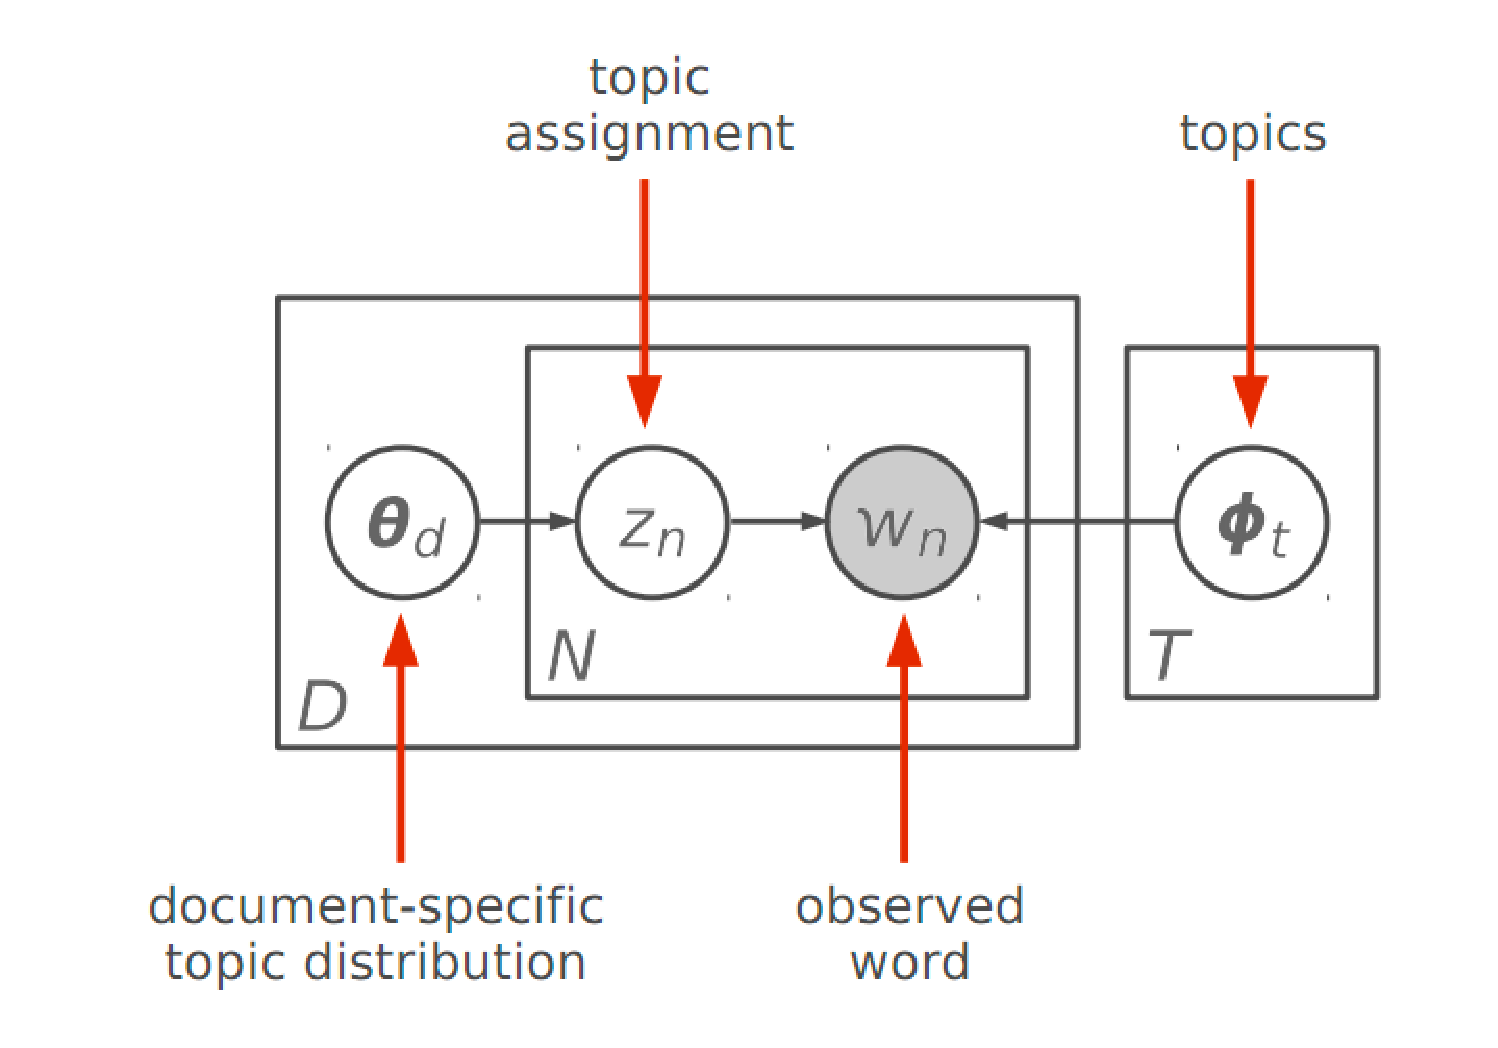
\includegraphics[width=400px]{figures/LSA.eps}
  \caption{The PLSA model}
  \label{fig:plsa}
\end{figure}

A significant step forward in this regard was made by Hofmann, who presented the probabilistic LSA (PLSA) model, where the mixture components are multinomial random variables that can be viewed as representation of “topics”~\cite{hofmann1999probabilistic}. Thus each word is generated from a single topic, and different words in a document may be generated from different topics. Each document is represented as a list of mixing proportions for these mixture components and thereby reduced to a probability distribution on a fixed set of topics. This distribution is the ``reduced description'' associated with the document. The PLSA model attempts to relax the simplifying assumption made in the mixture of unigrams model that each document is generated from only one topic. In a sense, it does capture the possibility that a document may contain multiple topics. 

\\
\item Latent Dirichlet allocation

Latent Dirichlet allocation (LDA) is a generative probabilistic model of a corpus and proposed by Blei David. The basic idea is that documents are represented as random mixture over latent topics, where each topic is characterized by a distribution over words. In LDA, it assumes the following generative process for each document to generate the words:

\begin{itemize}
\item Randomly choose a distribution over topics.

\item For each word in the document

  \begin {itemize}
\item Randomly choose a topic from the distribution over topics in step 1.
\item Randomly choose a word from the corresponding distribution over the vocabulary.
  \end{itemize}
\end{itemize}
\begin{figure}[!htb]
  \centering
  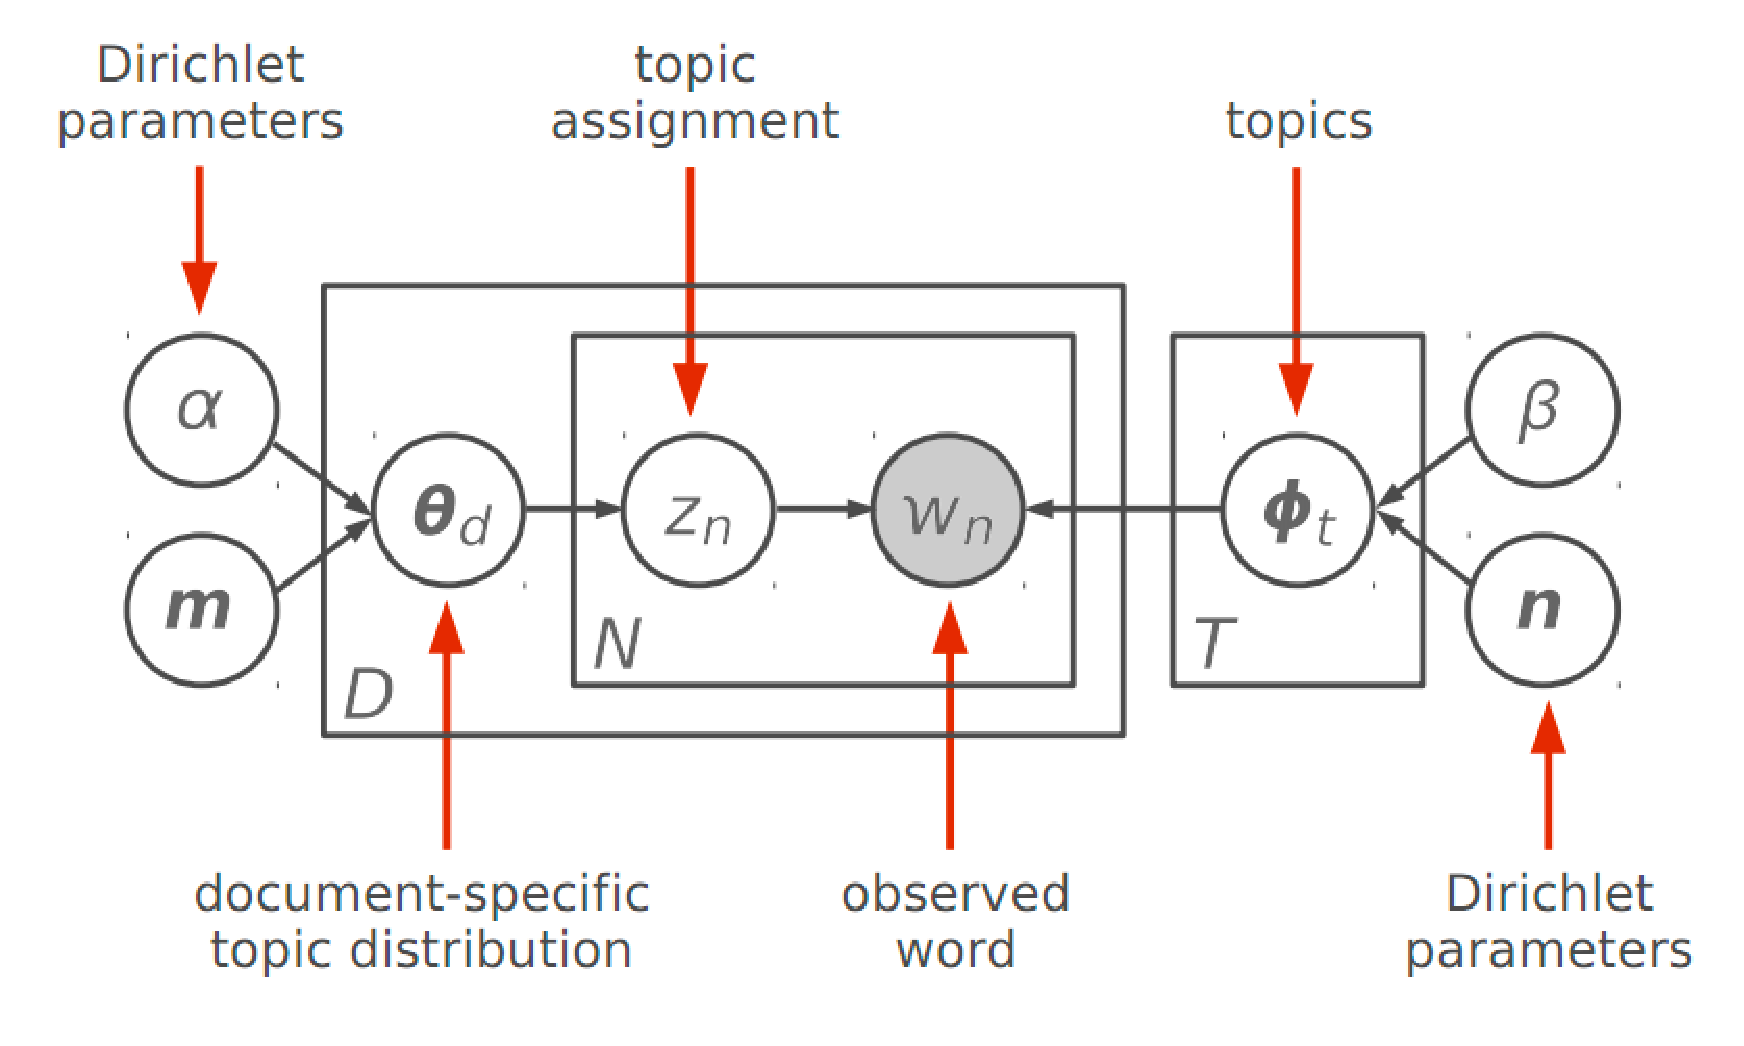
\includegraphics[width=400px]{figures/LDA.eps}
  \caption{The graphical model for latent Dirichlet allocation. Each node is a
random variable and is labeled according to its role in the generative
process. The hidden nodes–the topic
proportions, assignments and topics—are unshaded. The observed
nodes—the words of the documents—are shaded. The rectangles are
``plate" notation, which denotes replication. The N plate denotes the
collection words within documents; the D plate denotes the collection
of documents within the collection.}
  \label{fig:lds}
\end{figure}

This statistical model reflects the intuition that documents exhibit multiple topics. Each document exhibits the topics with different proportion; each word in each document is drawn from one of the topics, where the selected topic is chosen from the per-document distribution over topics. 
 
\end{itemize}

\section{Topology construction}
For some social medias, there are explicit social networks on which the information is diffused. This type of social medias includes the Twitter (the node represents the user, and the directed edge represents the following-followed relationship), Facebook (the node represents the user, and the undirected edge represents the friendship), etc. For the other social medias, we can only observe that one is got infected without knowing who infect it. This type of social medias includes the news websites and the personal blogs. We call this kind of topology construction prolem as network inference problem.

In~\cite{gomez2010inferring}, Gomez-Rodriguez et al. described this problem as: given a hidden directed network $G*(V,E*)$, where the set of $E*$ is unknown. Also for every node $v_i$, we know a triple tuple $(v_i,t_i,\Phi_i)$, which means at time $t_i$, $v_i$ is infected with a set of features or attributes $\Phi_i$. We aim to solve an optimization problem to find the set of $G*$. They built on the independent cascade model (See Chapter 4) and decribed the optimization problem as $$\hat{G} = argmax\limit_{|G|\le k}P(C|G)$$ where the maximization is over all graphs $G$ of at most $k$ edges.

In~\cite{eagle2009inferring}, Eagle et al. infered the friedship network structure from the mobile data and claimed that it is possible to accurately infer 95\% friendship relations.

In addition, some techniques to be introduced in Chapter 5.3 can be used to solve this problem.

\section{Sentiment analysis}
When analyzing the information diffusion, a very important attribute we need know is in which attitude a person got infected. Take the Twitter as an exmple, the users can rewteet a tweet with their comments. In this case, we can analyze the users' attitudes for the tweet by analyzing their comments. In~\cite{pang2008opinion}, Pang summaried 332 studies on opinion mining and sentiment analysis and classified the approaches into two categroies: the unsupervised approaches and supervised approaches. 

Among the unsupervised approaches, there ara a lot of studies on unsupervised lexicon induction, which is to create a sentiment lexicon in an unsupervised manner and use it to determine the degree of positivity of the content~\cite{hatzivassiloglou2000effects}~\cite{yu2003towards}. Bootstrapping is another unsupervised approach. The main idea is to generate the labeled data by using one available initial classifier~\cite{riloff2003learning}~\cite{wilson2005opinionfinder}. Moreover, Pang and Lee~\cite{thomas2006get} proposed a simple “blank slate” method based on the rarity of words within the search results that are retrieved. For the supervised approachs, they just use a collection of representative data to train a classifier. To compare these approaches, Chaovalit and Zhou did the comparing experiments on them~\cite{chaovalit2005movie}.








